\documentclass[notitlepage,twocolumn,nofootinbib,showpacs,preprintnumbers,superscriptaddress,amsmath,amssymb]{revtex4-1}
%\documentclass[notitlepage,nofootinbib,showpacs,preprintnumbers,superscriptaddress,amsmath,amssymb]{revtex4-1}
%\documentclass[notitlepage,nofootinbib,showpacs,preprintnumbers,superscriptaddress,amsmath,amssymb,11pt]{revtex4-1}

% Some other (several out of many) possibilities
%\documentclass[preprint,aps]{revtex4}
%\documentclass[preprint,aps,draft]{revtex4}
%\documentclass[prb]{revtex4}% Physical Review B

\usepackage{graphicx}% Include figure files
\usepackage{dcolumn}% Align table columns on decimal point
\usepackage{bm}% bold math
\usepackage{amsmath}
\usepackage{multirow}
%\usepackage{algorithm}

\newcommand{\astra}{{\sc Astra }}
\newcommand{\impactT}{{\sc Impact-T }}
\newcommand{\impactZ}{{\sc Impact-Z }}
\newcommand{\elegant}{{\sc Elegant }}
\newcommand{\astragenerator}{{\sc AstraGenerator }}
\newcommand{\mafia}{{\sc Mafia }}
\newcommand{\rmsemit}{\mbox{$\tilde{\varepsilon}$}}
\newcommand{\mean}[1]{\mbox{$\langle{#1}\rangle$}}
\newcommand{\matlab}{{\sc Matlab }}
\newcommand{\ud}{\mathrm{d}}

\usepackage[colorlinks=true]{hyperref}

%\nofiles
% MATH -----------------------------------------------------------
\newcommand{\norm}[1]{\left\Vert#1\right\Vert}
\newcommand{\abs}[1]{\left\vert#1\right\vert}
\newcommand{\set}[1]{\left\{#1\right\}}
\newcommand{\V}{\overrightarrow}
\newcommand{\N}{\hat}
\newcommand{\G}{\nabla}
\newcommand{\D}{\partial}
\newcommand{\Real}{\mathbb R}
\newcommand{\Int}{\mathbb N}
\newcommand{\eps}{\varepsilon}
\newcommand{\To}{\longrightarrow}
\newcommand{\BX}{\mathbf{B}(X)}
\newcommand{\A}{\mathcal{A}}
\newcommand{\re}{\mathcal{Re}}
\newcommand{\im}{{\cal Im}}
\newcommand{\T}{\mathbb{T}}
\newcommand{\dop}{\delta_{0p}}
\newcommand{\dom}{\delta_{0m}}
%


\usepackage{listings}

% Python style for highlighting
\newcommand\pythonstyle{\lstset{
        language=Python,
%        basicstyle=\ttm,
        otherkeywords={self},             % Add keywords here
%        keywordstyle=\ttb\color{deepblue},
        emph={MyClass,__init__},          % Custom highlighting
 %       emphstyle=\ttb\color{deepred},    % Custom highlighting style%
%        stringstyle=\color{deepgreen},
        frame=tb,                         % Any extra options here
        showstringspaces=false            % 
}}


% Python environment
\lstnewenvironment{python}[1][]
{
    \pythonstyle
    \lstset{#1}
}
{}


%\setlength{\oddsidemargin}{-3mm} \setlength{\evensidemargin}{-3mm}
\begin{document}
\title{Lattice settings for FAST}
%\thanks{ This work was partially sponsored by the the DOE contracts DE-SC00????? to Northern Illinois University 
%and DE-AC02-07CH11359 to the Fermi Research Alliance, LLC which operates Fermilab. }
%\author{P.  Piot} \affiliation{Northern Illinois Center for
%Accelerator \& Detector Development and Department of Physics,
%Northern Illinois University, DeKalb IL 60115,
%USA} \affiliation{Accelerator Physics Center, Fermi National
%Accelerator Laboratory, Batavia, IL 60510, USA}
%\author{M. Andorf} \affiliation{Northern Illinois Center for
%Accelerator \& Detector Development and Department of Physics,
%Northern Illinois University, DeKalb IL 60115,
%USA} \author{V. A. Lebedev} \affiliation{Accelerator Physics Center, Fermi National
%Accelerator Laboratory, Batavia, IL 60510, USA}
%\author{S. Chattopadhyay} \affiliation{Northern Illinois Center for
%Accelerator \& Detector Development and Department of Physics,
%Northern Illinois University, DeKalb IL 60115,
%USA} \affiliation{Accelerator Physics Center, Fermi National
%Accelerator Laboratory, Batavia, IL 60510, USA}
\date{\today}
	
\begin{abstract}
This Note summarizes a recipe to find a lattice setting in the {\sc fast} beamline. This is a first pass for comments. {\em Note: the lattice downstream of the HE dogleg could be improved further}.  
\end{abstract}
\preprint{PP, V2}
\maketitle
%
\section{Overview}

All the \elegant files are located in the main directory {\tt Elegant\_10132016\_Run}. The subdirectory {\tt All\_Lines\_old} contains the beamline lattice assembled by Dan. While the subdirectory {\tt All\_Line\_Edited} has the same beamlines with a few edits (mainly the addition of fit-point markers and the change in the quadrupole location ahead of dipole {\tt D600}). The following \elegant command files are contained in the main directory. 
\begin{itemize}
\item {\tt  injector\_cryo.ele}: beamline from $z=8$~m from cathode to cryomodule exit (gate valve GV418), the BC1 bunch compressor is turned off
\item {\tt  injector\_BC1\_cryo.ele}: beamline from $z=8$~m from cathode to cryomodule exit (gate valve GV418), the BC1 bunch compressor is turned on
\item {\tt cryotoFODOend.ele}: beamline from cryomodule exit (gate valve GV418) to FODO end (BPM B502). It is used to find the settings of quadupole magnets in the FODO channel and upstream the FODO. 
\item {\tt  FODOend\_todump.ele}: beamline from FODO end to HE dump. It is used to find the settings of quadupole magnets downstream of the FODO channel, in the dispersive section, and in the line up to the HE dump. 
\item {\tt  injectortodump.ele}: this files takes an incoming distribution at $z=8$~m and track up to the HE dump. 
\end{itemize}


To check the results the following script can be ran
\begin{itemize}
\item {\tt workflow}: fit all the quadrupole magnets (running the \elegant command files in the proper sequence) and display the resulting betatron function along the bunch compressor 
\item {\tt  clean\_directory}: erase all the \elegant output files. 
\end{itemize}

For all the calculation the incoming Courant-Snyder parameters are taken from an incoming particle distribution. In the current case I take an \impactT simulated distribution at $z=8$~m provided by Daniel Mihalcea (it corresponds to $Q=200$~pC).  Finally, in all calculations the quadrupoles Q106, Q107, and Q111 are assumed to be turned off as the planned to be skewed in support to flat-beam experiments. \\

\section{lattice fitting with Elegant}

\subsection{Case of BC1 compressor OFF}
When the compressor is turned off the following philosophy is used to devise the quadrupole settings in the injector (done in {\tt  injector\_cryo.ele}). First the beamline {\tt INJ\_PCM} (see {\tt LINE.lte} in {\tt All\_Line\_Edited} is used. The quadrupole magnets Q108, Q109, Q110, Q112 and Q113 are used to realize a waist at X118 (where a slit-based emittance measurement is available) while maintainin the betratron function  $\beta_{x,y}<50$~m over the full beamline. The downstream quadrupoles Q118, Q119, Q120, Q126, Q127, Q128 are devised to ensure the betratron function downstream of the cryomodule is divergent with an approximate betatron function $\beta_{x,y}\simeq 25$~m the corresponding betratron slope is taken to $\alpha_{x,y}\simeq -2$. The initial distribution is then tracked through the injector and the corresponding outputs {\tt  injector\_cryo.*} can be examined. The injector settings (parameter file) and Courant-Snyder evolution are available in respectively the {\tt injector.param} and {\tt injector.twi} files. The final distribution is saved in {\tt cryomodule\_end.out}.\\


The lattice downstream of the cryomodule up to the end of the {\tt ACM} line is fitted using the {\tt cryotoFODOend.ele}. First a unit-cell of the FODO channel (here called {\tt FODO\_ACM} is used to find the periodic solution and corresponding quadrupole settings for a given phase advance (in the current file I took $\nu_x=\nu_y=0.25$. This also provide the matched beta function saved in {\tt fodo.twi}. In the next step, the quadrupole upstream of the FODO channel
Q441, Q442, Q443, Q444 are fitted to match the incoming distribution Courant-Snyder parameters to the FODO cell parameters. Lastly the {\tt ACM\_to\_EIDstart} assembled the section downstream of the cryomodule and up the the start of the {\tt EID} line and track the distribution {\tt cryomodule\_end.out} up to the {\tt EID} line starting point. The beamline parameters are saved in {\tt acm.param} and the corresponding Courant-Snyder parameters are in {\tt acm.twi} 

Finally, the lattice up the the HE dump is worked out in the {\tt FODOend\_todump.ele}. First the quadrupole magnets within the dogleg (D600-D604) are fitted to ensure the dispersion and dispersion slope are all vanishing $\eta_x={\eta'}_x=0$ downstream of D604. The dispersion is also tweaked to be close to zero in the middle of Q602 [Note that Q602 is nominally exited to a large value (via the {\tt alter\_element} command) devised after a couple of iterations with the next step].  In a second step the upstream quadrupole Q502\_EID, Q503\_EID, Q504\_EID, Q505\_EID are fitted to provide a betatron function with small excursion and symmetrized with respected to the middle of the dogleg. During the process the previously devised value of the dogleg quadrupole Q601, Q602, and Q603 are slightly tweaked to ensure the dispersion and its slope remained to zero downstream of D604. Finally the quadupoles Q604, 605, 609, Q611, and Q612 are fitted to provide a large betatron function at the final dump window.  The beamline parameters are saved in {\tt eid\_epd.param} and the corresponding Courant-Snyder parameters are in {\tt eid\_epd.twi}. 

To validate the devised settings the \elegant file {\tt injectortodump.ele} is ran. The file used the beamline {\tt INJ\_EPD}. This file load all the parameters files that were created during the fitting process above and track the distribution from $z=8$~m to the HE dump window. The betratron and dispersion functions are shown in Fig.~\ref{CS1} and  ~\ref{CS2} respectively while the beam size evolution appears in Fig.~\ref{rms}. 
%
\begin{figure}[hhhh!!!]
\begin{center}
 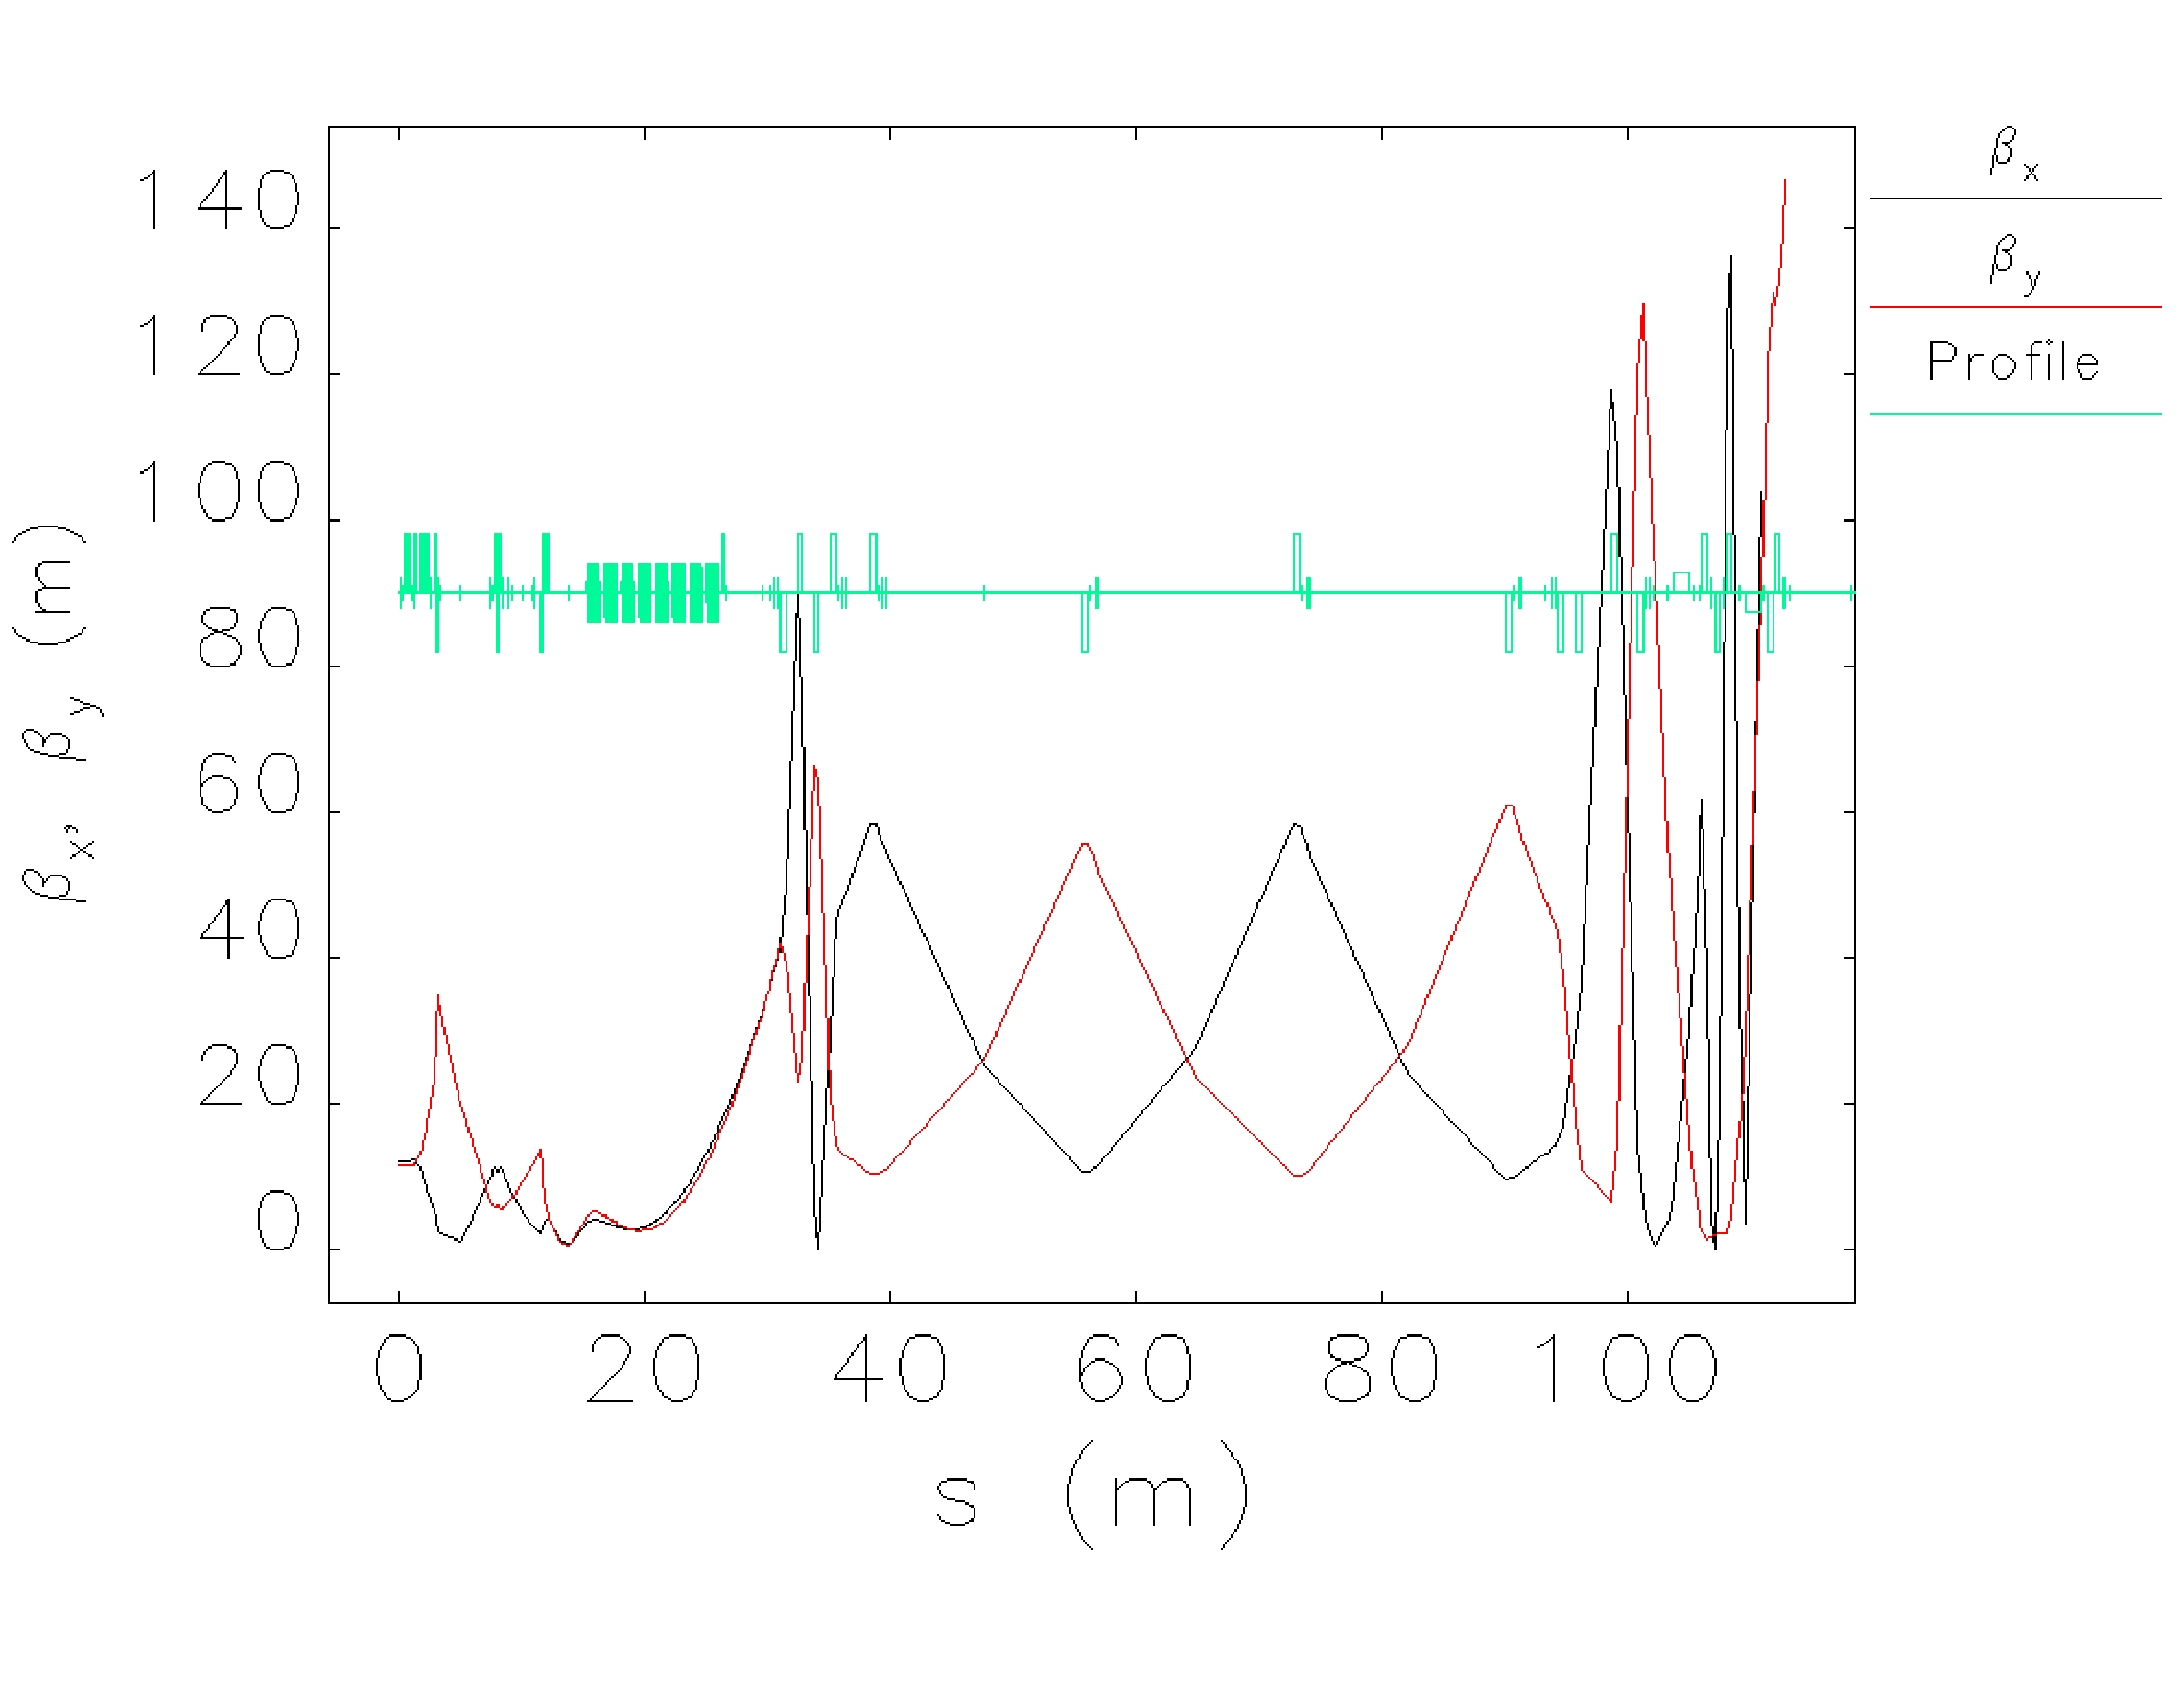
\includegraphics[width=0.95\linewidth]{injectortodump_twiss.pdf}
\caption{Betatron function evolution along the FAST injector (the ordinate $s=0$ correspond to $z=8$~m from the photocathode). Note that betatron function value in excess of 150~m are not displayed for clarity.\label{CS1} }
\end{center}
\end{figure}
\begin{figure}[hhhhh!!!!]
\begin{center}
 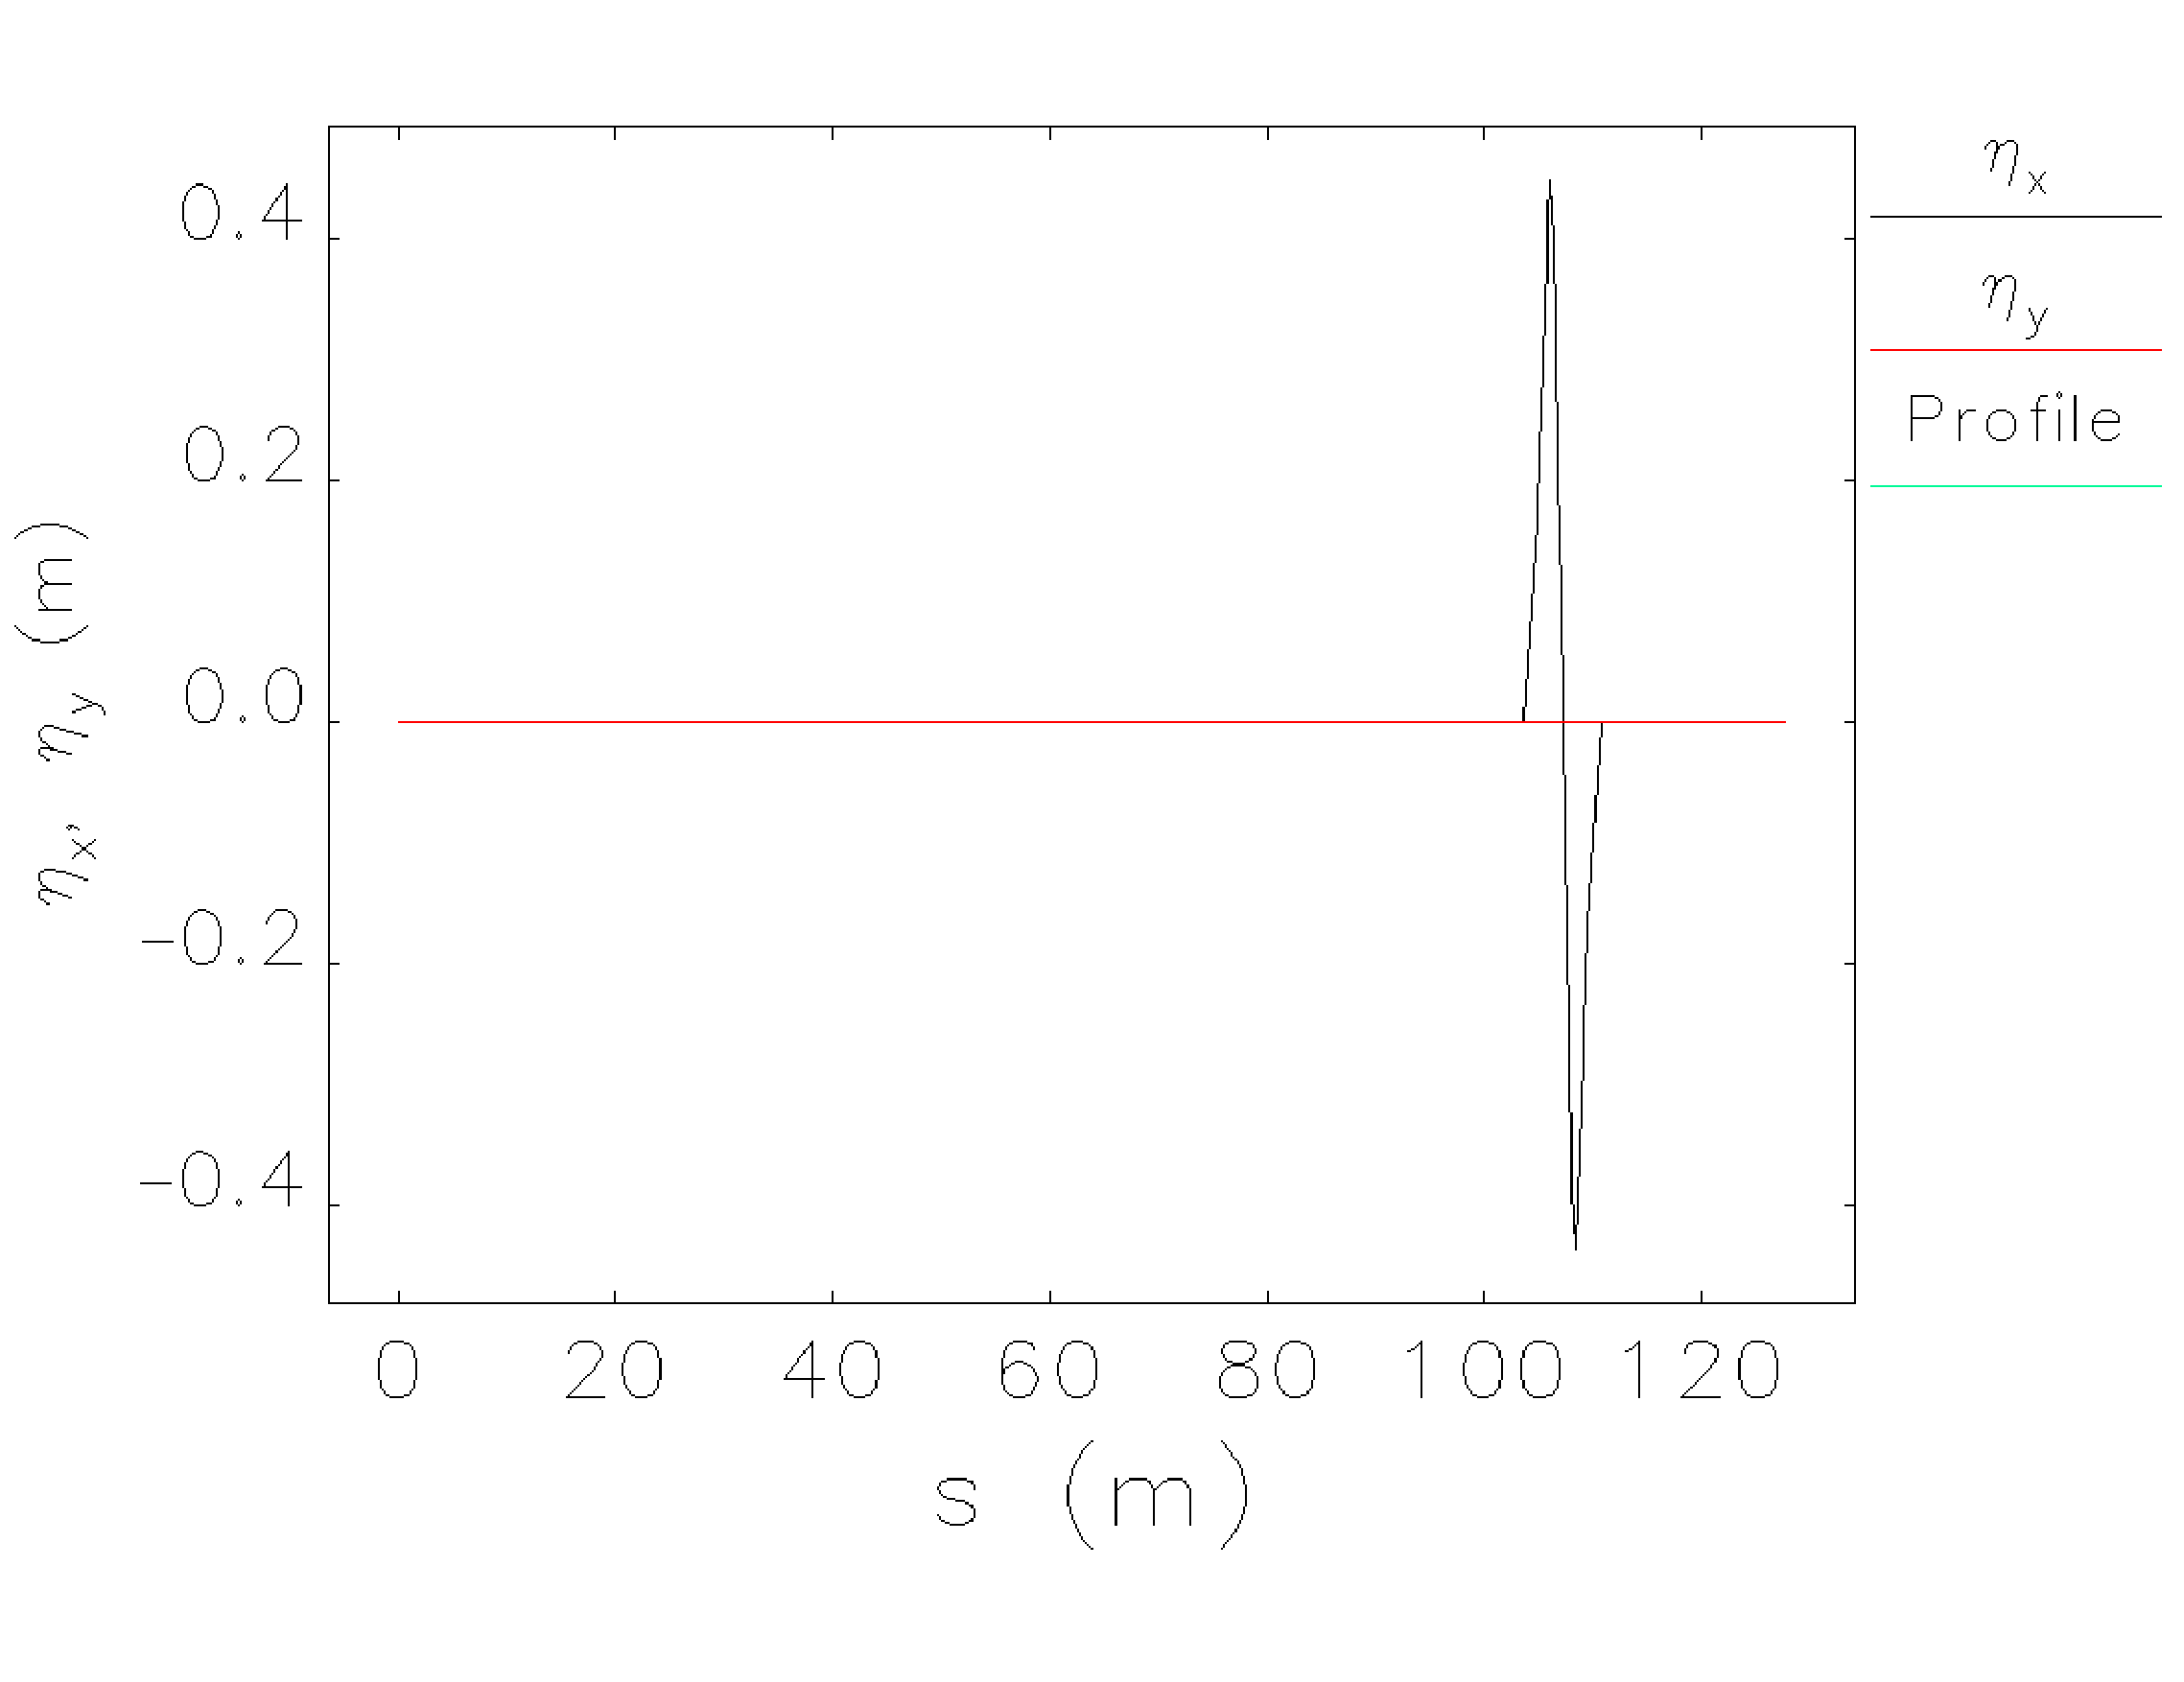
\includegraphics[width=0.95\linewidth]{injectortodump_eta.pdf}
\caption{Dispersion function evolution along the FAST injector (the ordinate $s=0$ correspond to $z=8$~m from the photocathode). \label{CS2} }
\end{center}
\end{figure}

\begin{figure}[hhhhh!!!!]
\begin{center}
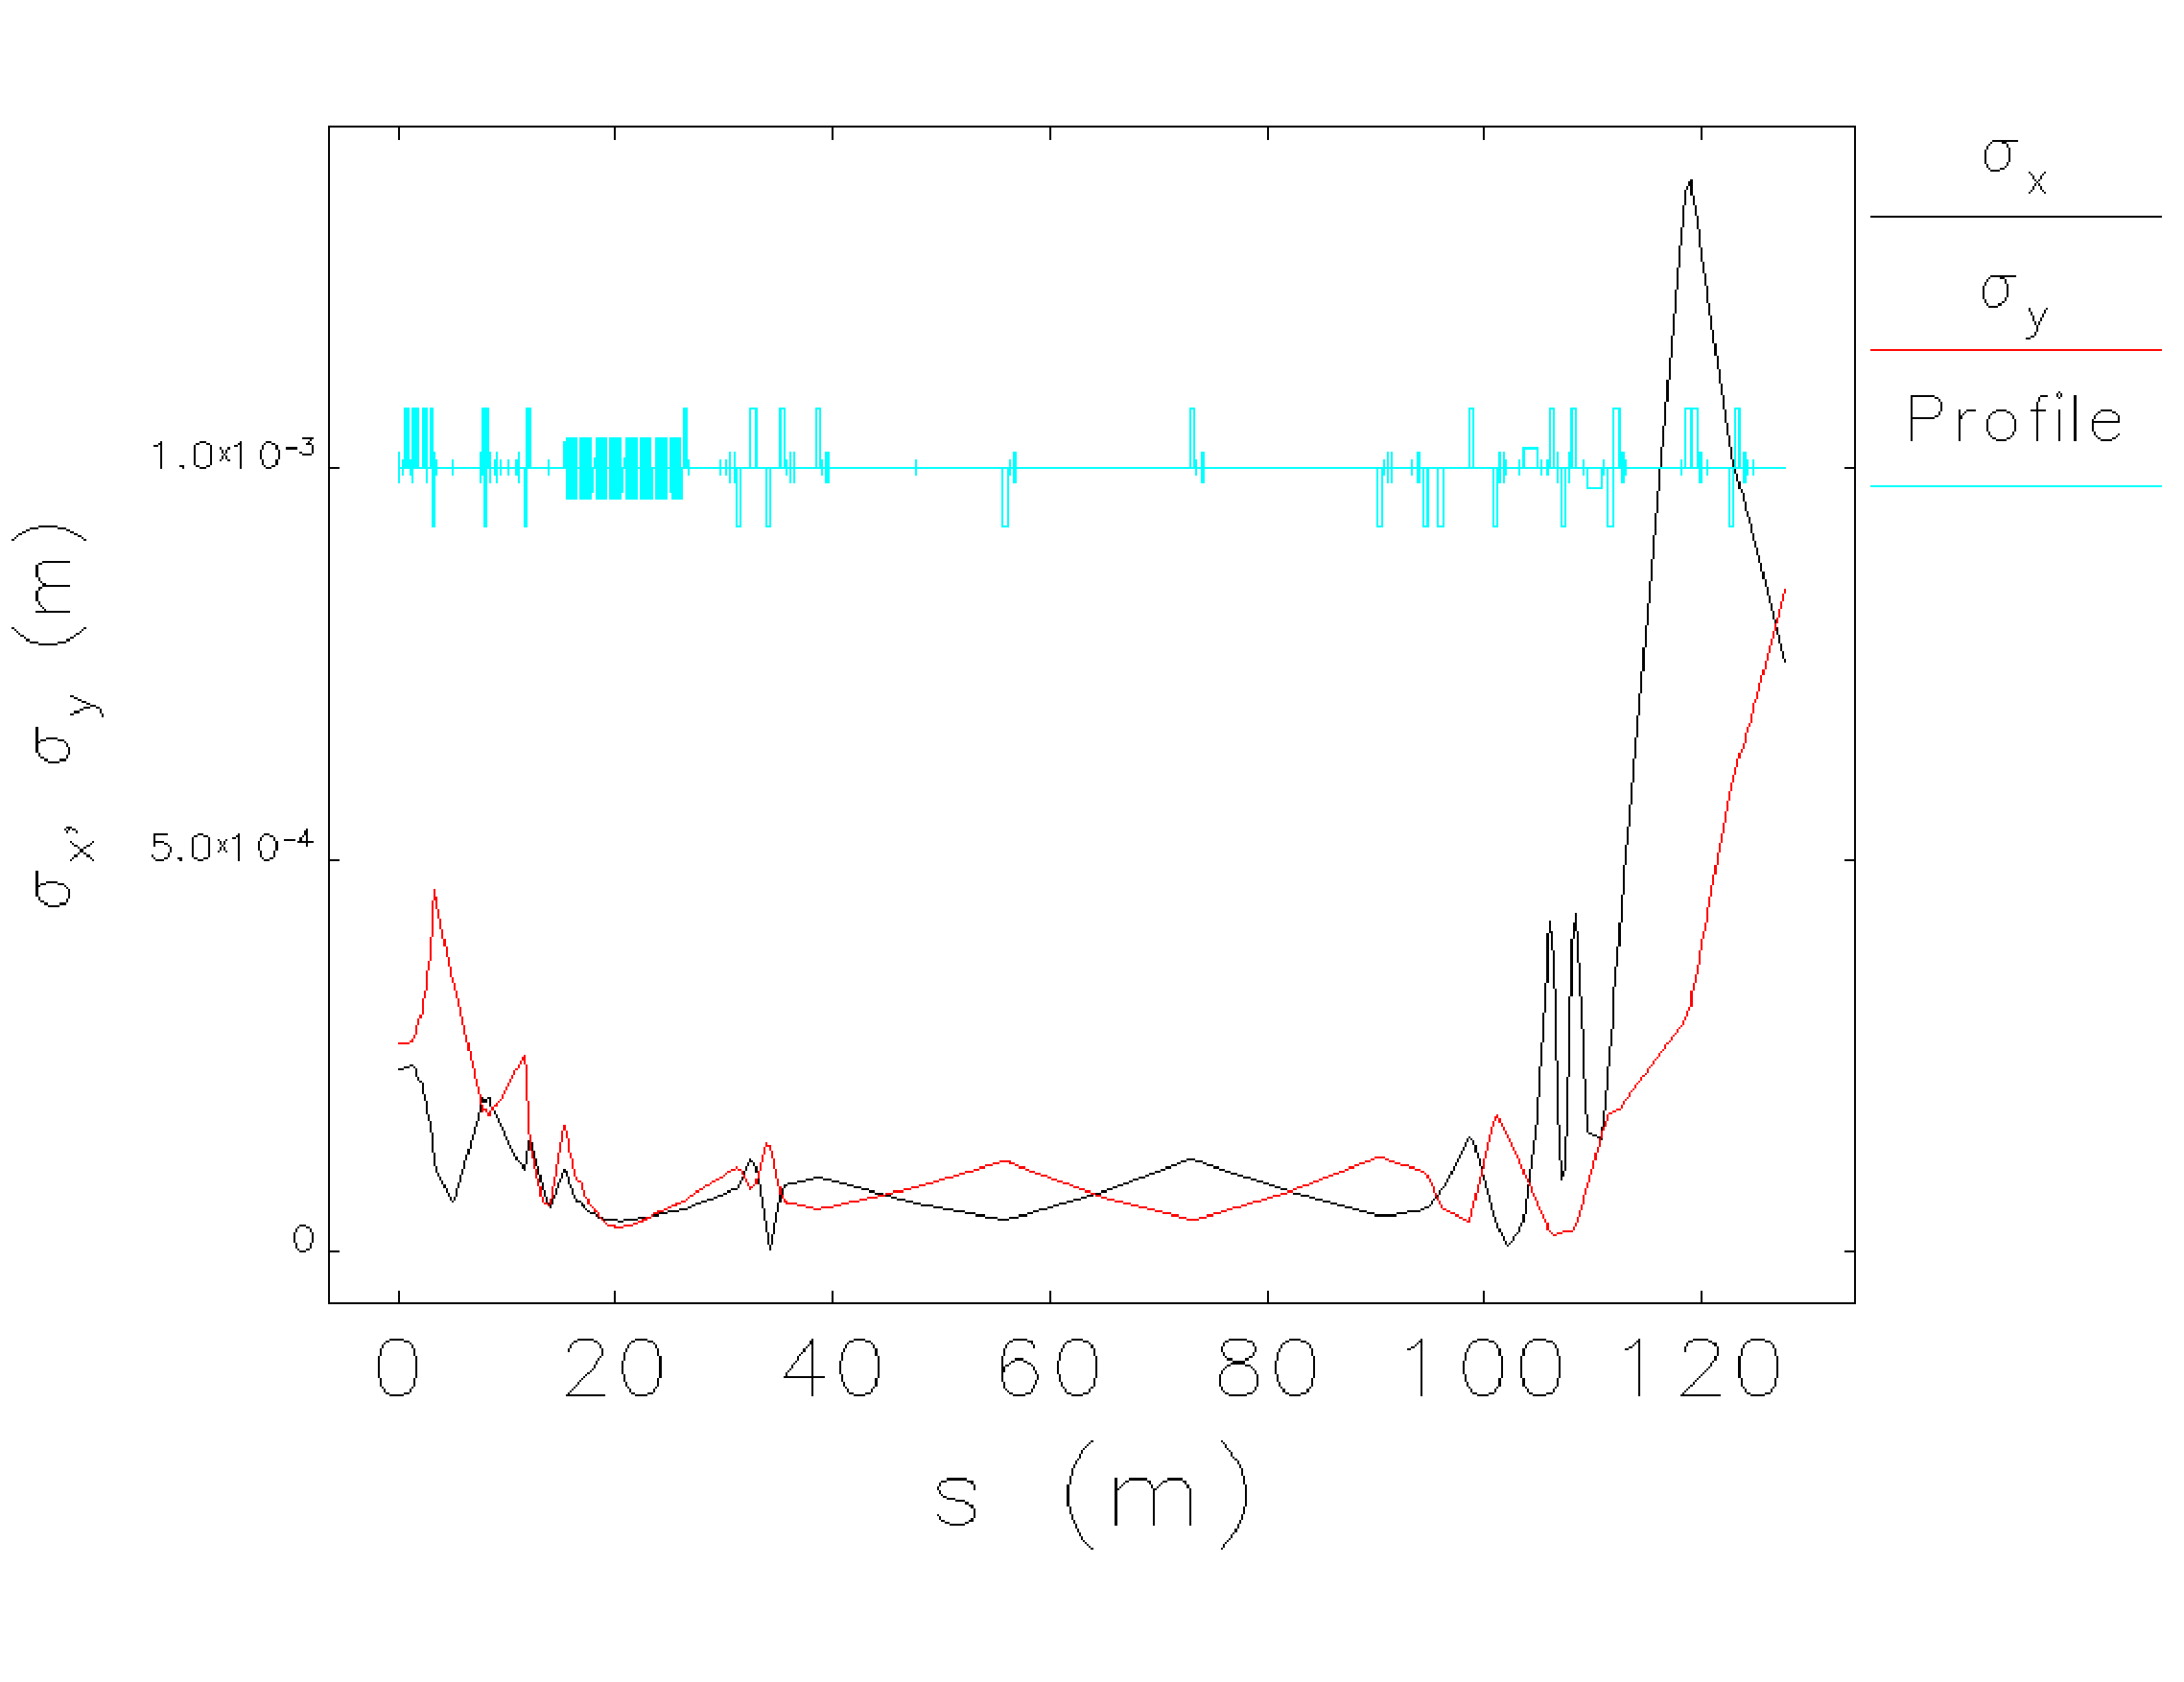
\includegraphics[width=0.95\linewidth]{injectortodump_rms.pdf}
\caption{Transverse ms beam size evolution along the FAST injector (the ordinate $s=0$ corresponds to $z=8$~m from the photocathode). \label{rms} }
\end{center}
\end{figure}
%
\subsection{Case of BC1 compressor ON}
%
The same procedure as detailed in the previous section is used to devise the quadupole settings when the BC1 compressor is turned on. The main difference lies in the injector beamline. The file {\tt  injector\_BC1\_cryo.ele} follows a similar workflow as {\tt  injector\_cryo.ele} except for the fitting of quadrupole magnets Q108, Q109, Q110, Q112 and Q113 which are now used to realize a waist between the third and fourth dipole magnets of BC1. Such a waist was shown to minimize emittance dilution due to an induced energy spread while the beam is compressed (such an energy spread may results from longitudinal space charge or coherent synchrotron radiation effects). The parameter- and final-distribution filename produced by {\tt  injector\_BC1\_cryo.ele}  are identical to those generated by {\tt  injector\_cryo.ele}  so the fit of the following beamline is identical to the one detailed above. 
%
\begin{figure}[hhhh!!!!!!!!!!!!!!!]
\begin{center}
 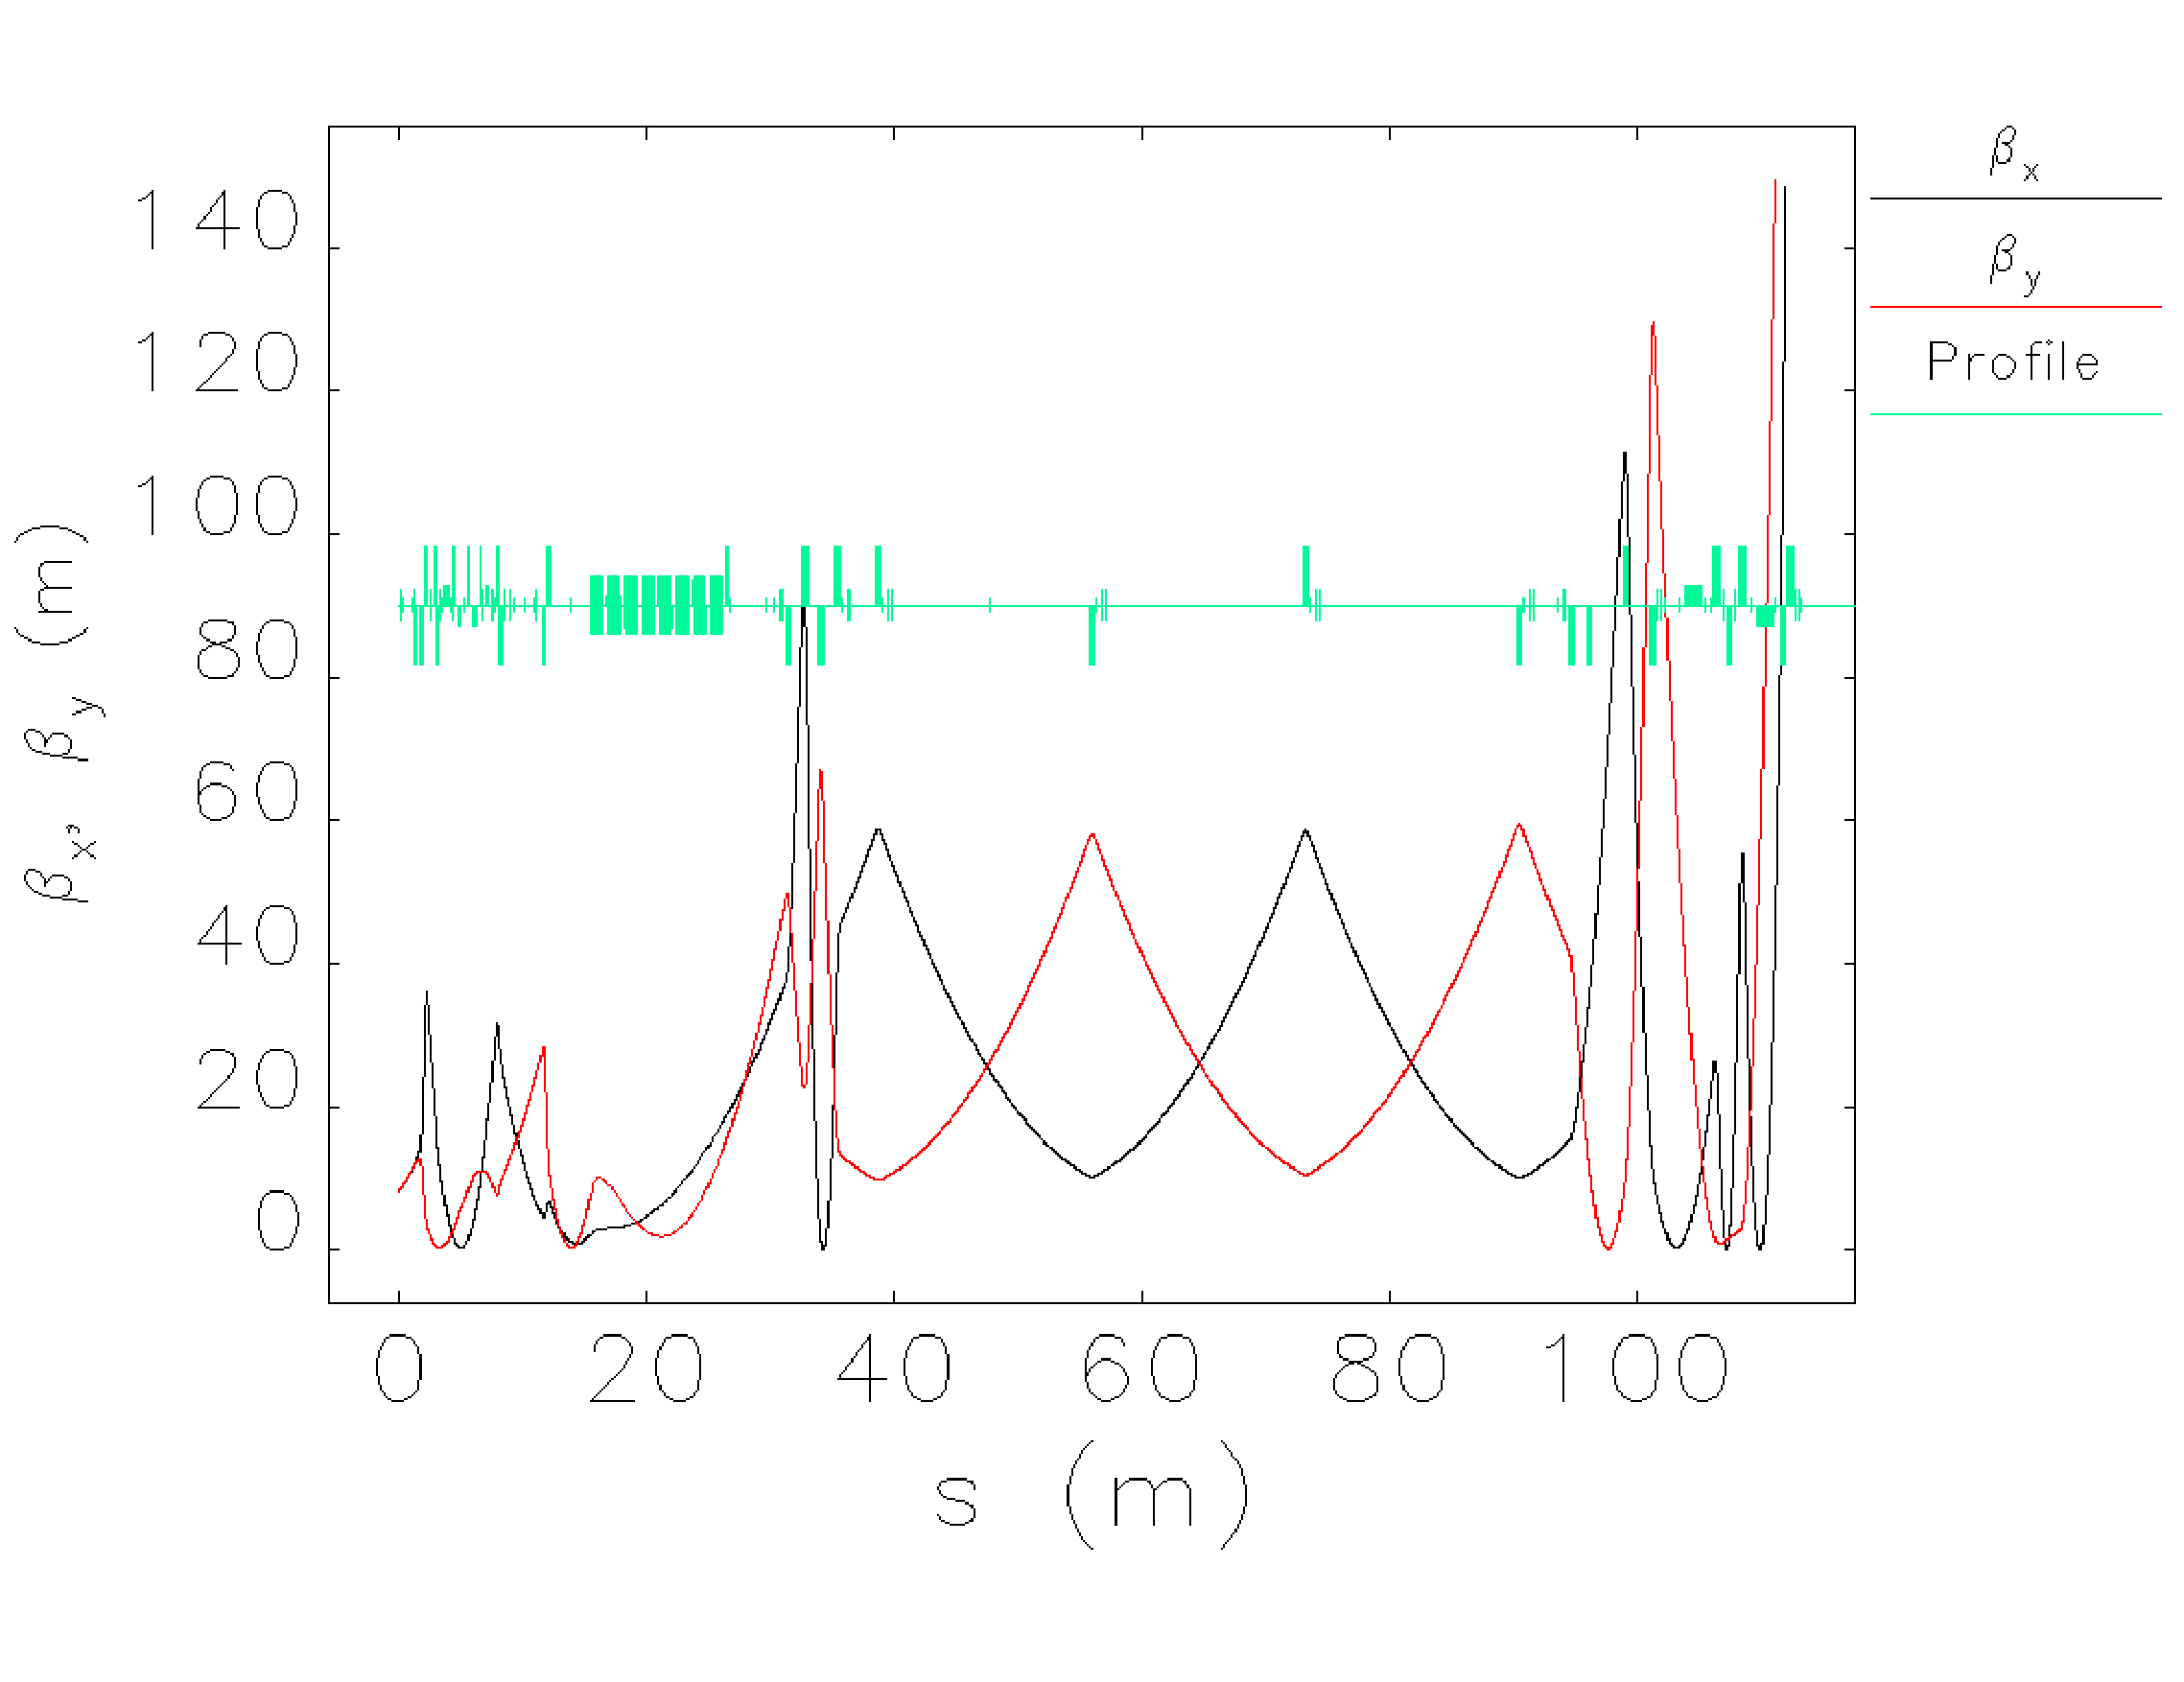
\includegraphics[width=0.95\linewidth]{injectortodump_twissbc.pdf}
\caption{Betatron function evolution along the FAST injector with BC1 turned on (the ordinate $s=0$ correspond to $z=8$~m from the photocathode). Note that betatron function value in excess of 150~m are not displayed for clarity.\label{CS1bc} }
\end{center}
\end{figure}

To validate the devised settings the \elegant file {\tt injector\_BC1\_todump.ele}  should be used instead of {\tt injectortodump.ele}; the former file now use the beamline {\tt INJ\_BC1\_EPD}.  The corresponding betatron and dispersion functions are shown in Fig.~\ref{CS1bc} and  ~\ref{CS2bc} respectively while the beam size evolution appears in Fig.~\ref{rmsbc}. 

\begin{figure}[hhhh!!!!!!!!!!!!]
\begin{center}
 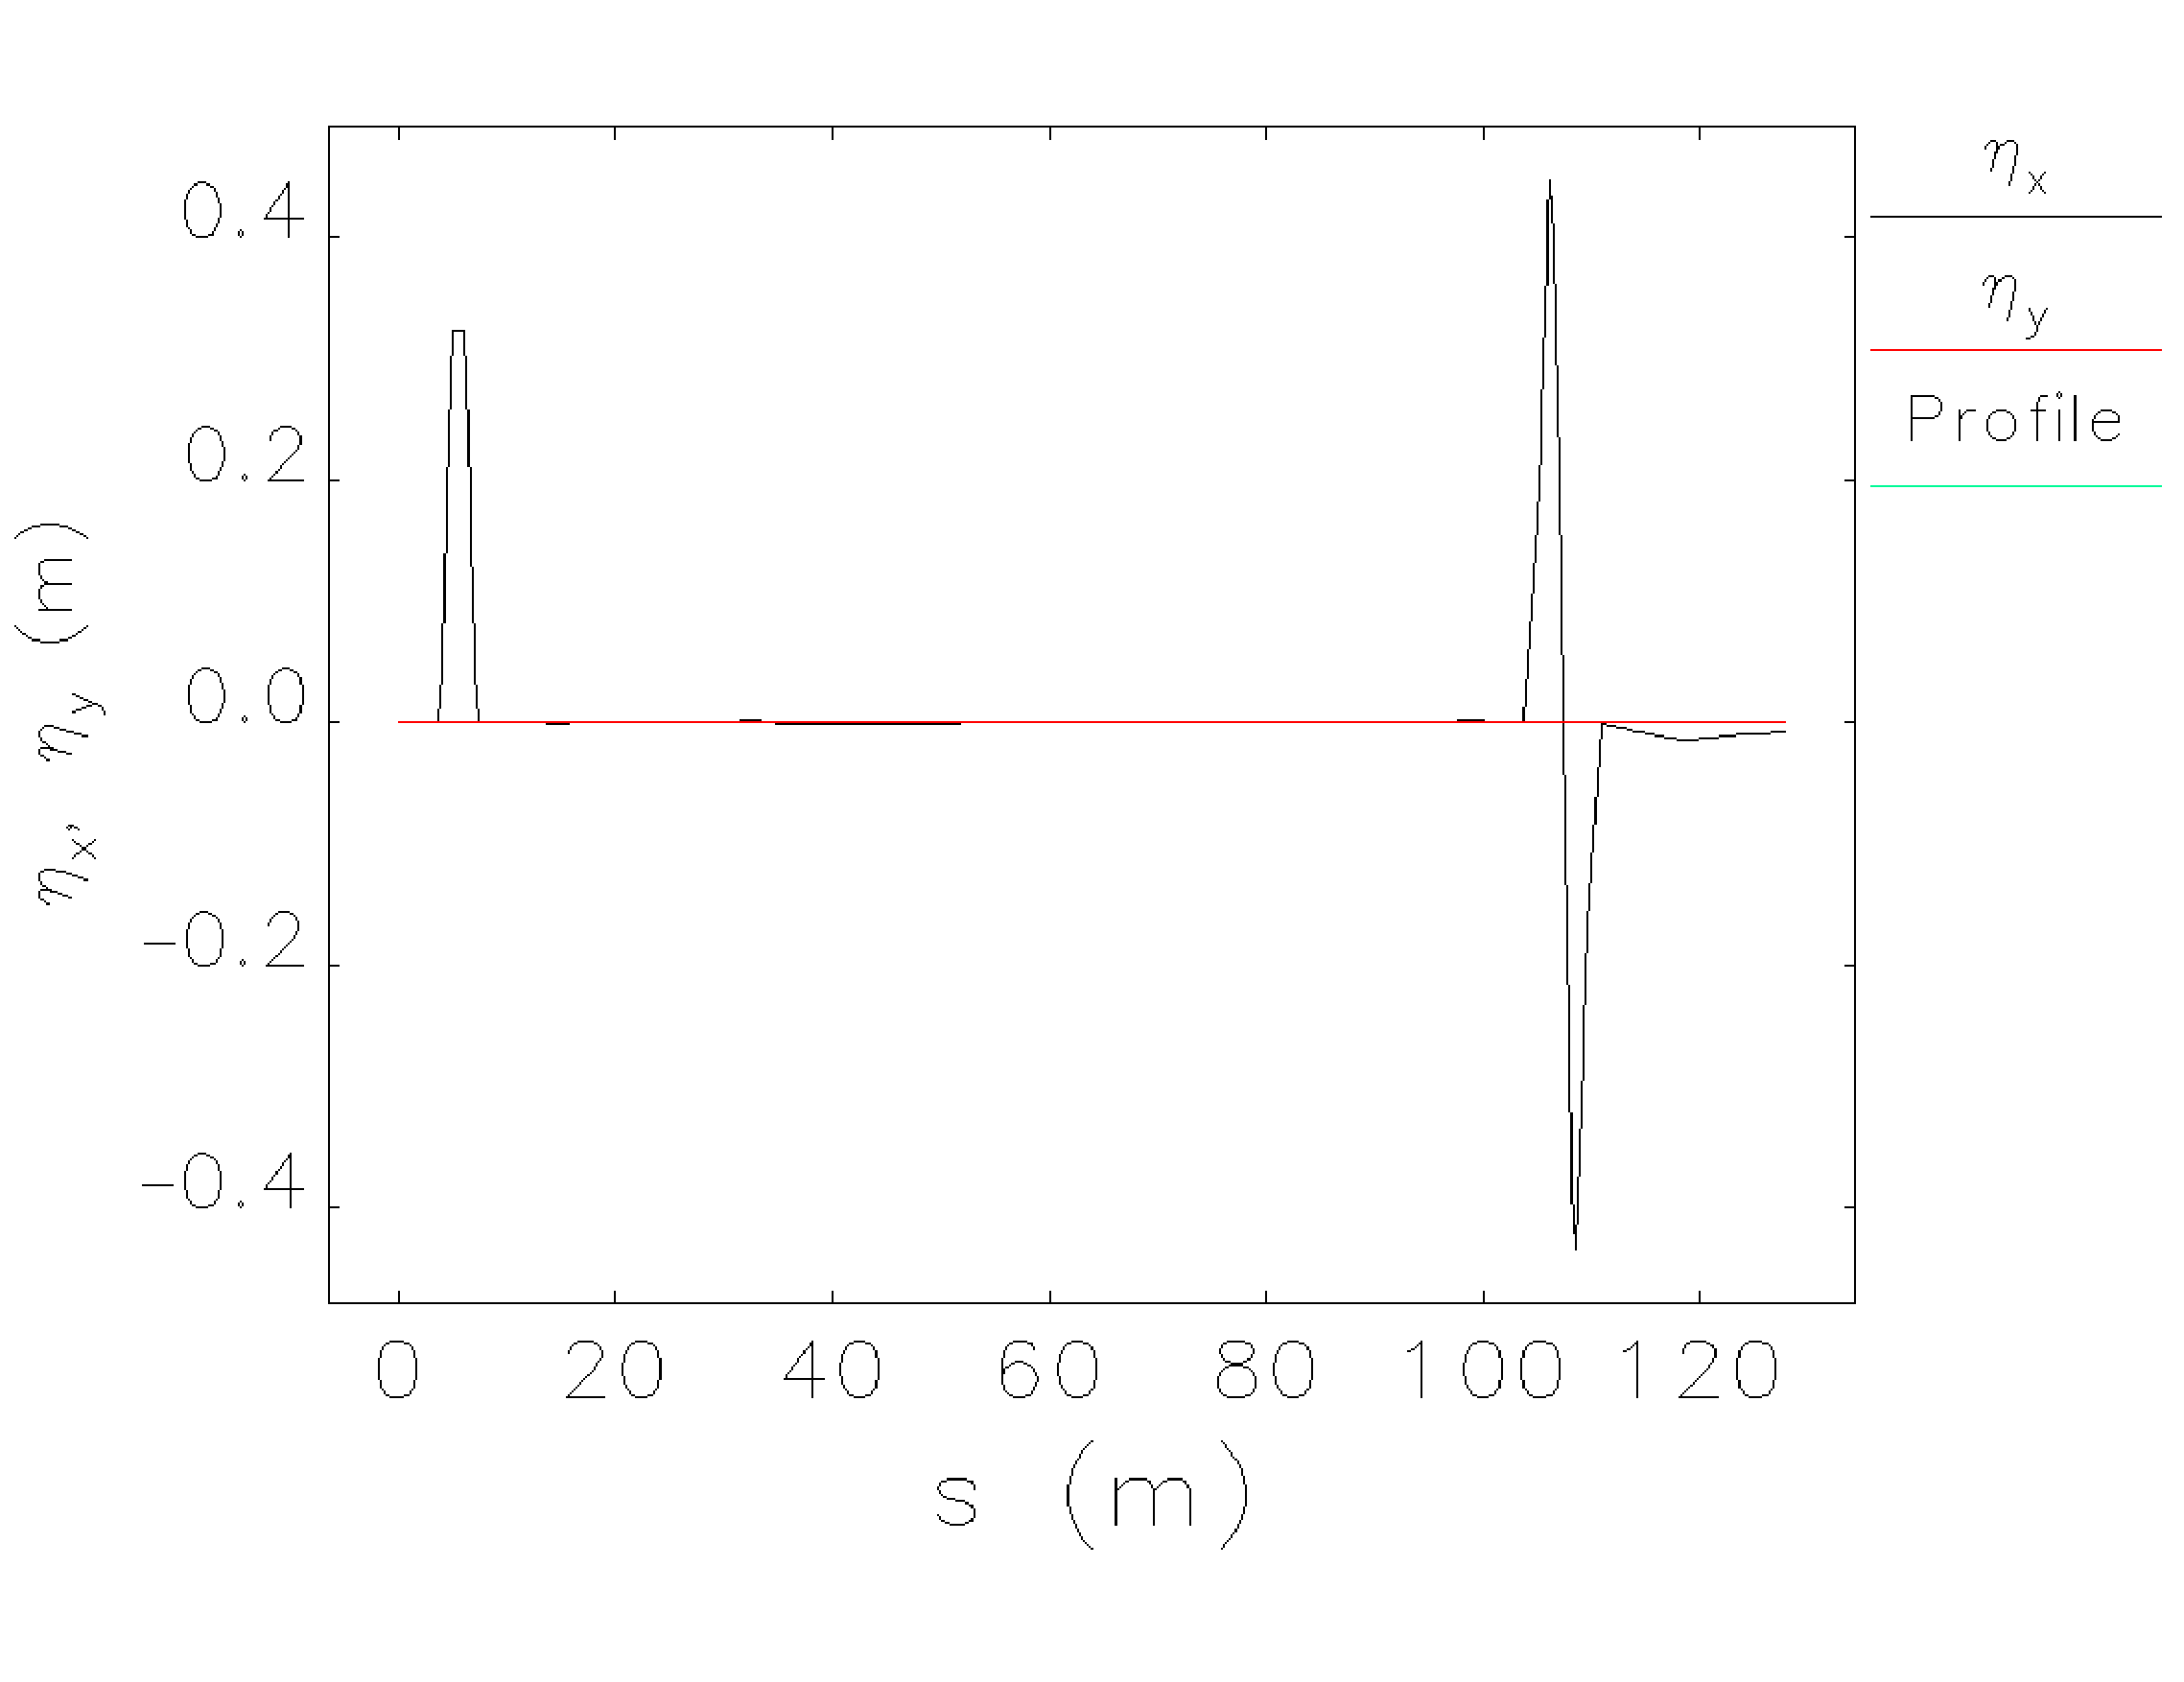
\includegraphics[width=0.95\linewidth]{injectortodump_etabc.pdf}
\caption{Dispersion function evolution along the FAST injector with BC1 turned on (the ordinate $s=0$ correspond to $z=8$~m from the photocathode). \label{CS2bc} }
\end{center}
\end{figure}
\begin{figure}[hhhh!!!!!!!!!!]
\begin{center}
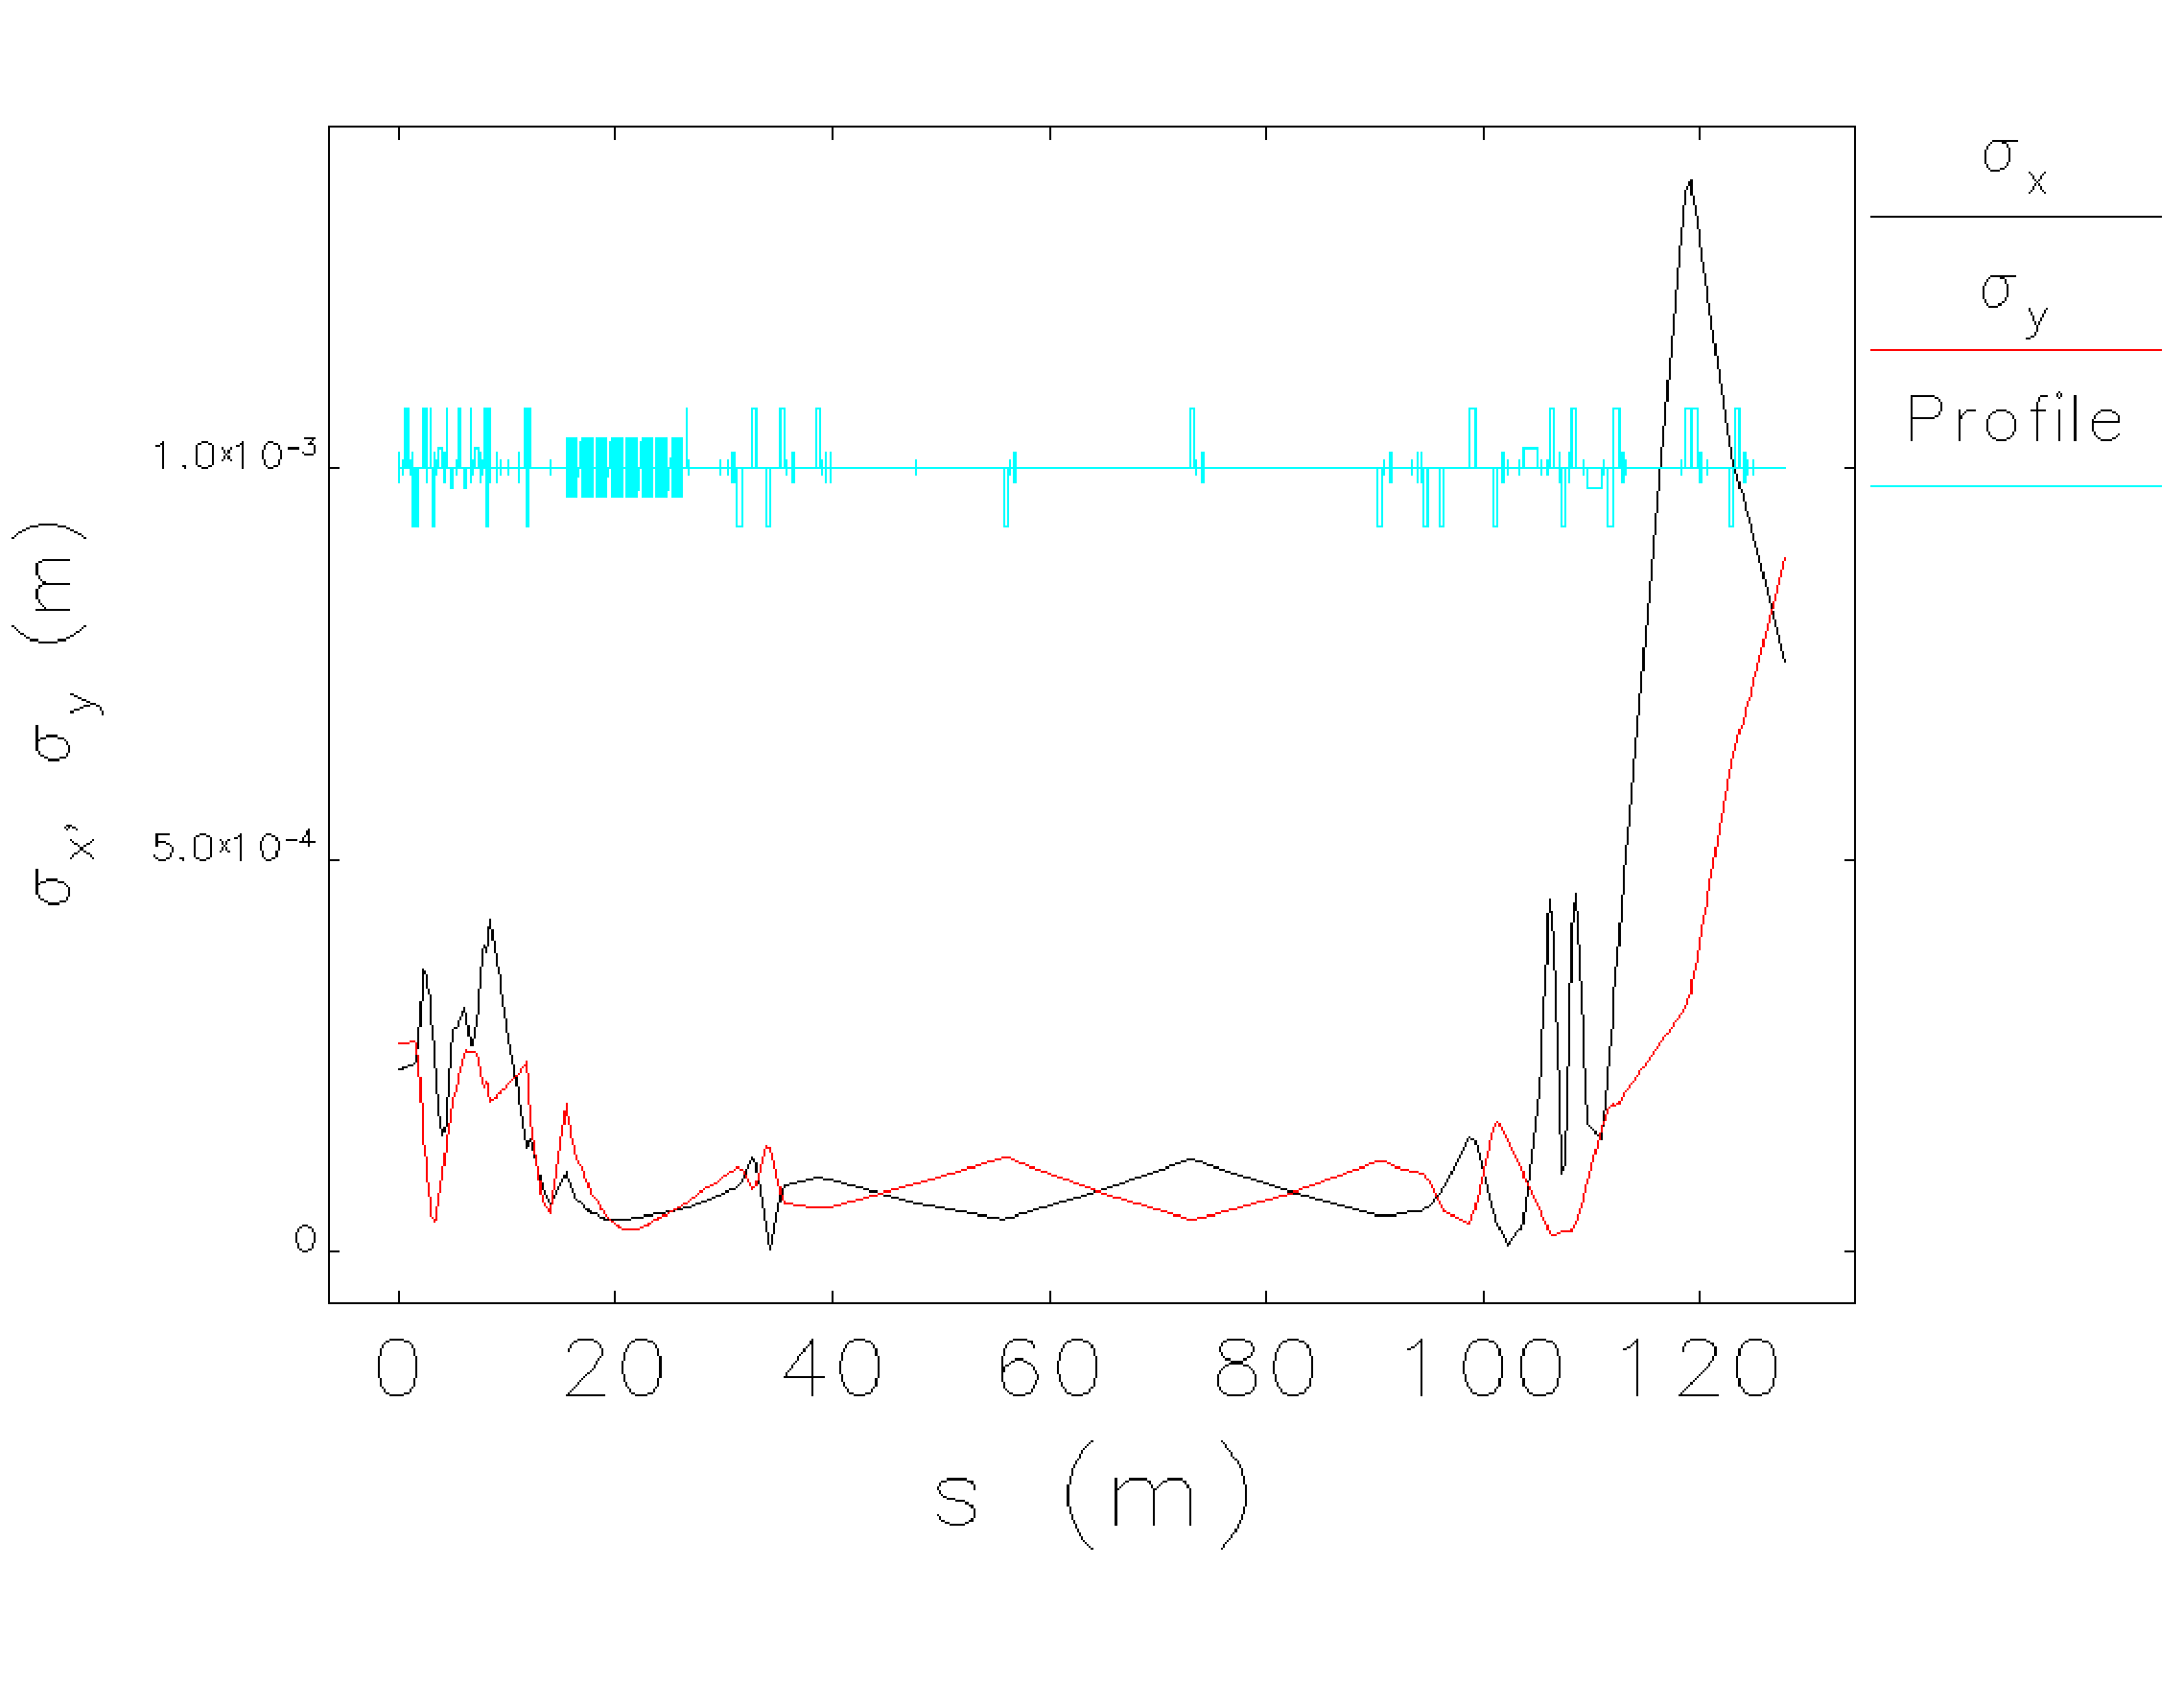
\includegraphics[width=0.95\linewidth]{injectortodump_rmsbc.pdf}
\caption{Transverse ms beam size evolution along the FAST injector with BC1 turned on (the ordinate $s=0$ corresponds to $z=8$~m from the photocathode). \label{rmsbc} }
\end{center}
\end{figure}
 %
\section{Impact-Z tracking}
%
The generated lattice can be directly converted into an \impactZ input deck so that tracking including space charge and CSR can be performed. This section outlined the conversion procedure. The output lattice from  {\tt injector\_BC1\_todump.ele} or  {\tt injectortodump.ele} under the same filename {\tt injectortodump.saved\_lattice}, likewise the survey file is save under {\tt injectortodump.survey}. The survey file needs to be converted to a text file as follows: {\tt sddsprintout -nolabel -notitle -column=s -column=ElementName -column=ElementType injectortodump.survey  $>$ currentSurvey }. Then the script {\tt ConvertElegant2ImpactZ.py} needs to be edited with the relevant information and ran via the command {\tt python ConvertElegant2ImpactZ.py}. The output file {\tt impactz.lattice} contains the lattice in the \impactZ format~\footnote{In \impactZ the quadrupole magnet sign convention is opposite to \elegant}. 

%
%
%%%%%%%%%%%%%%%%%%%%%%%%%%%%
%
\end{document}

